\newpage
\section{Vorbereitung}
Informieren Sie sich über Timer-Interrupts in dem Dokument TivaWare$^{TM}$ Peripheral Driver Library und lesen Sie im Workbook\footnote{\url{http://software-dl.ti.com/trainingTTO/trainingTTO\_public\_sw/GSW-TM4C123G-LaunchPad/TM4C123G\_LaunchPad\_Workshop\_Workbook.pdf}} Lab 4 und Lab 6 nach.\\ \\
Schlagen Sie die entsprechenden Stellen für den Hibernation Mode im Workbook nach. Verwenden Sie die Schaltung gemä\ss{} dem Schaltbild 3. Verwenden Sie 150 $\Omega$ Widerstände. Für den Knopfdruck verwenden Sie den auf dem Board verbauten Knopf mit der Beschriftung SW2 (im Code $"$PUSH2$"$). Die Schaltung entspricht einem Aufbau einer Fu\ss{}gängerampel und einer Fahrzeugampel, wie man sie aus dem Stra\ss{}enverkehr kennt.\\
\begin{figure}[h]
	\centering
	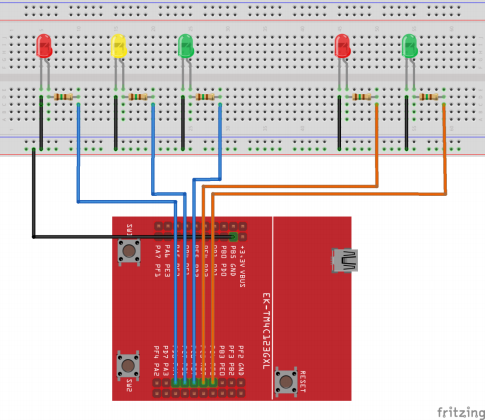
\includegraphics[width=0.9\linewidth]{images/Schaltbild3}
	\label{fig:Schaltblid3}
\end{figure}
\begin{center}
	Schaltbild 3
\end{center}
\newpage
\section{Aufgabe 1}
Die Funktionalität der Schaltung ist mittels des LaunchPads wie folgt umzusetzen:
\begin{itemize}
	\item Im Default-Zustand ist die Fahrzeugampel grün, die Fu\ss{}gängerampel rot. 
	\item Mit einem Knopfdruck startet nach dem Ablauf einer ersten Zeitspanne ($T_w$) eine Umschaltsequenz der Ampeln. Diese Sequenz beginnt mit der Umschaltung der Fahrzeugampel von grün über gelb auf rot. Danach erfolgt eine Umschaltung der Fu\ss{}gängerampel von rot auf grün. Jede Umschaltung dauert dabei eine zweite Zeitspanne ($T_u$). Nach einer dritten Zeitspanne ($T_g$) schalten die beiden Ampeln zurück. Diesmal erfolgt zuerst das Umschalten der Fu\ss{}gängerampel von grün auf rot, dann der Fahrzeugampel von rot über gelb-rot auf grün. Jede Umschaltung der Ampeln dauert dabei wieder die zweite Zeitspanne ($T_u$).
\end{itemize}
Modellieren Sie das gewünschte Verhalten des Systems mittels eines Statecharts.\\
\begin{figure}[h]
	\centering
	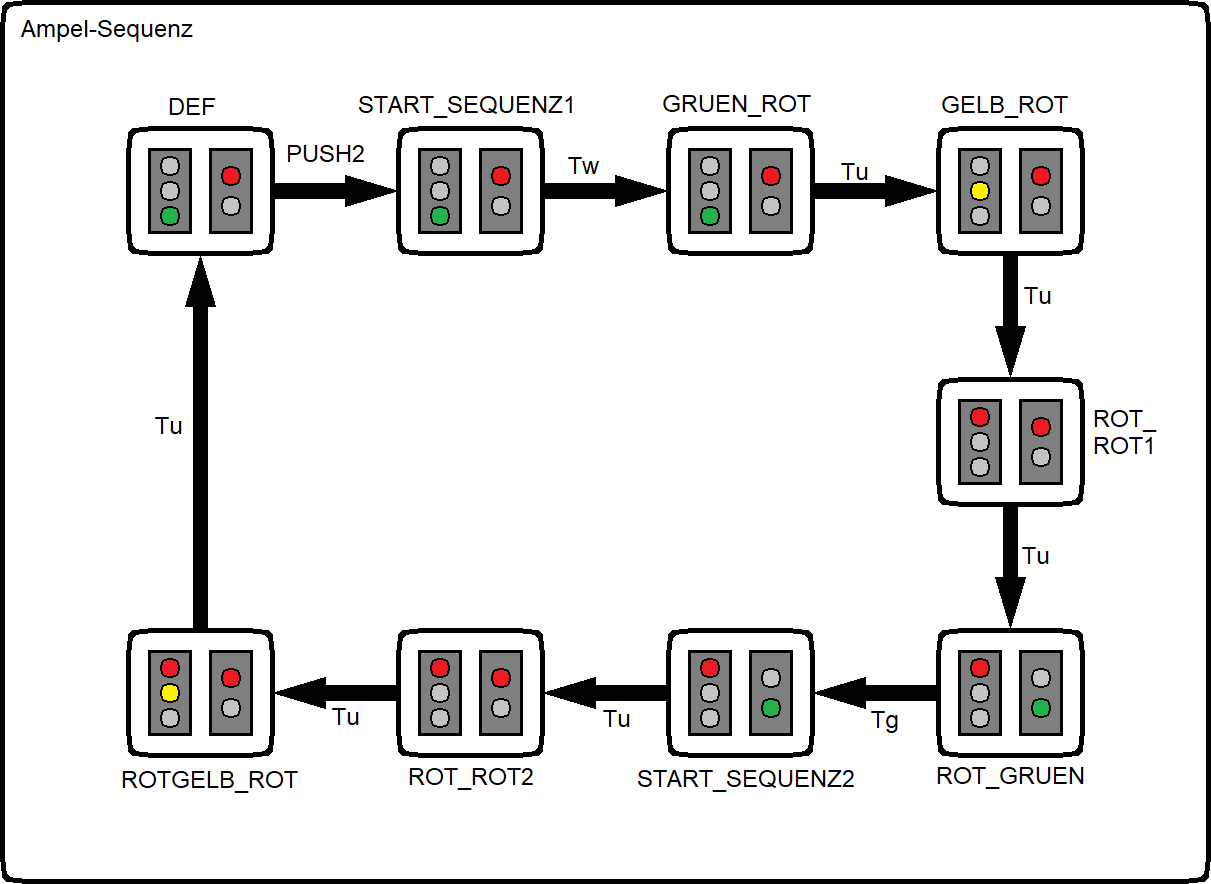
\includegraphics[width=0.7\linewidth]{images/Statechart}
\end{figure}
\begin{itemize}
	\item PUSH2: Button SW2 wurde gedrückt.
	\item Tw: Zeitspanne Tw ist abgelaufen.
	\item Tu: Zeitspanne Tu ist abgelaufen.
	\item Tg: Zeitspanne Tg ist abgelaufen.
\end{itemize}
Implementieren Sie ausgehend von Ihrer Modellierung deren Funktionalität. Ihre Modellierung der Zustände muss in der Implementierung klar wieder zu finden sein. Die Verwendung von Timer-Interrupts ist für diese Aufgabe nicht erforderlich.\\ \\
\definecolor{mygreen}{rgb}{0,0.6,0}
\definecolor{mymauve}{rgb}{0.58,0,0.82}
\lstset{
	breakatwhitespace=false,
	breaklines=true,
	commentstyle=\color{mygreen},
	frame=single,
	keepspaces=true,
	showstringspaces=false,
	keywordstyle=\color{blue},
	language=C,
	rulecolor=\color{black},
	stringstyle=\color{mymauve},
	tabsize=2
}
\newpage
\noindent Klasse Led:
\lstinputlisting[firstline=26, lastline=43]{../Aufgabe1/Aufgabe1.ino}
\noindent Klasse Button:
\lstinputlisting[firstline=45, lastline=59]{../Aufgabe1/Aufgabe1.ino}
\noindent Ampeln:
\lstinputlisting[firstline=61, lastline=70]{../Aufgabe1/Aufgabe1.ino}
\noindent Zustände:
\lstinputlisting[firstline=12, lastline=22]{../Aufgabe1/Aufgabe1.ino}
\noindent Implementierung Statechart
\lstinputlisting[firstline=24, lastline=24]{../Aufgabe1/Aufgabe1.ino}
\lstinputlisting[firstline=81, lastline=143]{../Aufgabe1/Aufgabe1.ino}
\newpage
\section{Aufgabe 2}
Fügen Sie dem Zustandsautomaten und dem Programm aus Aufgabe 1 die Eigenschaft hinzu, dass das Board (und die Ampeln) nach einer Zeit ($T_e$) ohne Knopfdruck in einen Energiesparmodus geht, aus welchem es bei Knopfdruck aufwacht. Der Energiesparmodus darf nur erreicht werden, wenn die Fahrzeugampel grün (und die Fu\ss{}gängerampel rot) ist. Dabei sollen auch alle LEDs ausgeschaltet werden.\\ \\
Verwenden Sie für diese Aufgabe einen Timer-Interrupt. Schreiben Sie dazu eine Klasse \textit{Timer}, die intern den Timer-Interrupt benutzt. Die Klasse \textit{Timer} muss u.a. die Methoden \textit{setTimer}(Zeitspanne) und \textit{resetTimer}() bereitstellen. Der Ablauf einer mit \textit{setTimer}(Zeitspanne) eingestellten Zeitspanne muss bei der Ereignisverarbeitung benutzt werden. Implementieren Sie für die Klasse \textit{Timer} das Singleton-Pattern, so dass nur eine Instanz der Klasse \textit{Timer} existiert. Die Funktion ISR für den Timer-Interrupt kann au\ss{}erhalb der Klasse \textit{Timer} sein. Die Funktion ISR kann über das Singleton-Pattern auf die Timer-Klasse zugreifen.\\
Statt die Interrupt Vector Tabelle zu ändern, wie es im Workbook gemacht wird, verwenden Sie die Funktion $"$TimerIntRegister$"$ von Tiva (siehe Driver Lib Doku).\\ \\
Das Programm darf nicht die Funktion \textit{delay}() der Energia-Bibliothek verwenden. Sämtliche Zeitabläufe sind über die Klasse Timer durchzuführen.\\
Für die Zeitspannen soll gelten: $T_e > T_w \geqq T_g > T_u$. Die Zeitspannen sollen auf halbe Sekunden genau einstellbar sein.\\ \\
Tipp: Sollte sich das Board beim Entwickeln nicht mehr flashen lassen, so ist es wahrscheinlich noch im Energiesparmodus. Starten Sie das Board neu, drücken Sie den SW2-Button (das Board verlässt den Energiesparmodus) und flashen Sie das Board.\\
\begin{figure}[h]
	\centering
	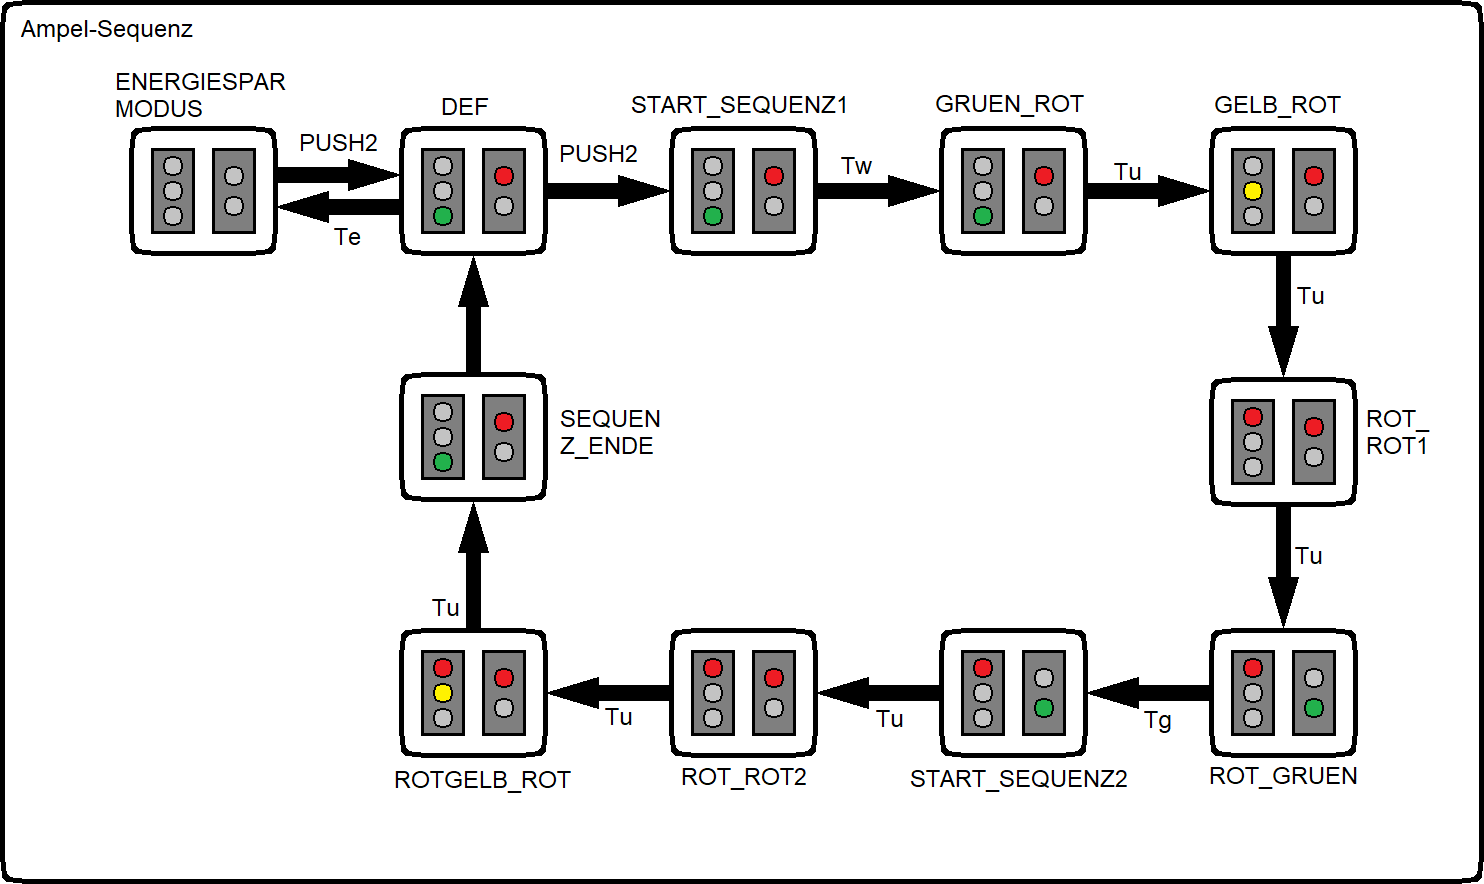
\includegraphics[width=0.7\linewidth]{images/Statechart2}
\end{figure}
\begin{itemize}
	\item PUSH2: Button SW2 wurde gedrückt.
	\item Tw: Zeitspanne Tw ist abgelaufen.
	\item Tu: Zeitspanne Tu ist abgelaufen.
	\item Tg: Zeitspanne Tg ist abgelaufen.
	\item Te: Zeitspanne Te ist abgelaufen.
\end{itemize}
\noindent Klasse Timer:
\lstinputlisting[firstline=88, lastline=135]{../Aufgabe2/Aufgabe2.ino}
\noindent Zustände:
\lstinputlisting[firstline=20, lastline=32]{../Aufgabe2/Aufgabe2.ino}
\noindent Implementierung Funktion ISR:
\lstinputlisting[firstline=137, lastline=247]{../Aufgabe2/Aufgabe2.ino}